\chapter{Literature Survey}

This section will explain why there’s a need for this system by exploring background literature related to this subject. Mainly the need of a proper system to test scientific software, start with explaining what a scientific software is, following up by explaining why most of them are not tested correctly. Then we will be discussing the two main components of this system, Cucumber and Behave. Then finally, explaining what casual testing is, the main method used by this system to test other software, and exhibit why it lacks a proper interactive system for non software engineering users.

\section{Scientific software}
Using a computational model for scientific research is common practice with today’s technology, scientists use these models to predict the result of an experiment or the outcome of an event. But whether these models can accurately predict the result, is still a problem since most of them lack some form of proper testing. Below will be discussing what is a computational model and why they are poorly tested.
\subsection{Computational model}
What defines a scientific computational model, it’s by using computers to simulate and study real life events by using mathematics, statistics, physics, and computer science to study the mechanism and behavior of complex systems by computer simulation \cite{Reference1}. \\*\\*
By using models that contain a number of input variables, and algorithms that will define the system. These models will simulate real-life situations and researchers can adjust these models by changing their variable and algorithm according to the results to make the model more conform to reality. Then researchers can use these models to see how one or more variables can affect the outcome of a certain event. Computational models provided some level of prediction of being able to calculate an anticipated result from a given set of variables \cite{Reference4}. This forecasting system can be used to predict complex systems, such as weather or disease spread, and help researchers or decision makers to decide their next move.\\*\\*
An example of this kind of model is Covasim \cite{Reference5}, Covasim uses agents to simulate individual people, the model mainly focused on one type of calculation, what is the probability of an individual in a given time step will change from not infected to infected, or badly ill to death. \\*\\*
The simulation starts from loaded the parameters, then it will start creating individual with different age, sex, and comorbidities based on the selected location (i.e., Different country). Then will be grouped into a social network depending on their attributes. After that the model will start looping, in each step, the model will apply various operations on the individual, then collect the result and apply analysis.

\subsection{Why computational models are hard to test}
Computational models are often very complicated, and require special knowledge related to the field. These models are often developed by scientists themselves, but most scientists aren’t software developers and may not have knowledge in some common software engineering practices, this may cost the quality of the scientific software \cite{Reference6}. Software testing is one of the aspects that is impacted, since the lack of knowledge in software development, lack of understanding in systematic testing is expected. Mistake can be made without notice and may affect the output of the system, causing the result to become inaccurate.\\*\\*
Testing a scientific software itself can be a difficult task to do, this may be the result of two types of challenges: \\*\\*
First is due to the software’s main purpose is to predict something unknown or simulate areas even researchers have little knowledge in, but to test a software, it is crucial to know how the software should Behave, what kind of output should it show. 
Without these knowledge, it is hard to tell if the software is working the right way. \\*\\*
Furthermore, these computation models are often consisting of hundreds of parameters and complex algorithm, this means it would require lots of test case in order to test every aspect of the system, and this leads high execution time making the testing process become very time consuming \cite{Reference6}.\\*\\*
Second is that scientific software is mostly developed with scientists being the lead role instead of a software engineer, and the value of the software system is often underestimated \cite{Reference6}. And most scientists never went through the training in software design like software engineer \cite{Reference7}, this means limited understanding of the testing process and not applying known testing methods. This will make the core design of the software unfriendly for effective testing.

\section{Current testing method}
Despite the difficulty in testing these models, there are still some common software testing methods that can be used to test them, such as behavior-driven development (or BDD) and Cucumber. Combined with casual model testing, a way to draw relationships between variables, it will make testing these complex models a lot easier.

\subsection{Behavior-driven development with Behave}
Behave is a python API based on behavior-driven development, behavior-driven development is a development technique that encourages collaboration between participants in a software project \cite{Reference8}. Behavior-driven development or BDD, aims to have a clear understanding of the desired software behavior between stakeholders and software developers, and communicate by writing test cases in a natural language that both sides can understand. Behave is a Python API created for this, it consists of tests written in Cucumber, an API written in natural language style. \\*\\*
When a test case is written, it requires a tool to read its specifications and see if the system works as the test-case specified. Cucumber is the tool that was developed for this purpose, it reads specifications written in plain text with a certain format and validates if the software does what those specifications say \cite{Reference9} and creates a report. \\*\\*
For Cucumber to understand the specifications, it must be written in Gherkin language, Gherkin uses a set of grammar and special keywords to give plain text structure so that Cucumber could understand it, one of the pros for Gherkin is that keyword can be translated to other languages, making it usable for people who don’t speak English \cite{Reference10}. \\*\\*
A proper Gherkin grammar starts by giving a context, then describing an event, and after that what should happen after the event. With these grammars, testers can specify a situation in the system, describe a certain parameter, and what the results should be with those parameters. By writing a test using Cucumber and Gherkin grammar, tester can combine them into a .Feature file as display below: 
\begin{figure}[h]
	\centering
	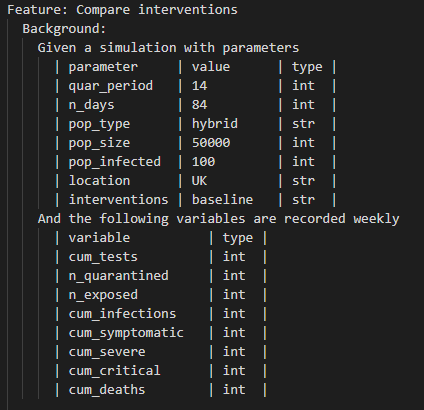
\includegraphics[width=10cm]{figures/featureFile.png}\\
	\caption{A feature file example.}
	\label{fig:figure1}
\end{figure}
\newpage \noindent With this .Feature file, tester can execute the file in terminal and Behave can read what needs to be tested and return a report.
\subsection{Causal testing}
With the help of Behave and Cucumber, we have the ability to test computational models. It is possible to test the entire system by writing an enormous feature file, but the execution time will become really long, and since computational models are usually in big scale it is also easy to make mistakes. This is when causal model can help simplify the testing process. \\*\\*
Causal model is a way to represent causal relationship within a system through mathematical model. It helps testers monitor causal relationships in the data \cite{Reference11}. A causal module can predict the behavior of a system, by comparing different inputs and the outputs a system produces, it can explore the cause and influence of a certain relationship \cite{Reference12}. By understanding these relationships, testers can test parts of the system by monitor if the inputs and outputs follow the same behaviour. \\*\\*
With this method testers can reduce the time required to test a complicated system by only testing parts of it one at a time, then combine the results, and testers can have a full picture of how the system performs. This is unlike the traditional method, where it requires testing the entire system all at once, and may require lots of time if it is a complicated system. \\*\\*

\subsection{Testing computational model with causal testing}
Causal testing can be a really useful testing method for software engineers \cite{Reference13}, however computational models are often developed by scientists or researchers who have limited knowledge in software testing \cite{Reference8}. Tester who wants to use causal model as a way to test system needs to have prior knowledge in how variables work in a software, this means people who may not have that much knowledge in software engineering, for example researchers in other fields, might not be able to conduct this method of testing in their software.

\section{Summary}

Behave is a powerful testing tool for software tester’s, based on the behavior-driven development method, encouraging people who do not specialize in software engineering to take part in testing. Assisted by Cucumber, a tool where users can describe testing steps in an easy-to-understand manner, and Cucumber compile and produce the results. With causal model, testers can effectively test large and complex computational models, saving time by only test parts of the system one at a time and combining the results together. But the problem is that when using causal model testing, it is inaccessible for most people, due to its lack of user-friendly nature. In order to make it more user friendly, we can integrate Cucumber and Behave with it to make it where users can use causal model testing by using Behave and Cucumber specify the testing process.
